% LaTeX Template for Project Report, Version 1.0

% Created by: Ernest Mwebaze
%Revised by: Azamuke Denish


\documentclass[12pt, a4paper]{article}
\usepackage{listings}
\usepackage[newfloat]{minted}
\usepackage{caption}
\usepackage{sidecap}
\usepackage{amsmath}


\newminted{python}{
\fontsize{9pt}
%
    % options to customize output of pythoncode
    % see section 5.3 Available options starting at page 16
}

\usepackage{xurl}
\usepackage[pdftex]{graphicx} %for embedding images
\usepackage{wrapfig}
\usepackage{hyperref}
\usepackage[font=scriptsize]{caption}
\usepackage{url} %for proper url entries
% \usepackage[bookmarks, colorlinks=false, pdfborder={0 0 0}, pdftitle={<pdf title here>}, pdfauthor={<author's name here>}, pdfsubject={<subject here>}, pdfkeywords={<keywords here>}]{hyperref} %for creating links in the pdf version and other additional pdf attributes, no effect on the printed document
%\usepackage[final]{pdfpages} %for embedding another pdf, remove if not required

\begin{document}
%\renewcommand\bibname{References} %Renames "Bibliography" to "References" on ref page

\pagenumbering{roman} %numbering before main content starts
%Include first stuff: title, acknowledgement, dedication, tables, etc
\begin{titlepage}

\begin{center}

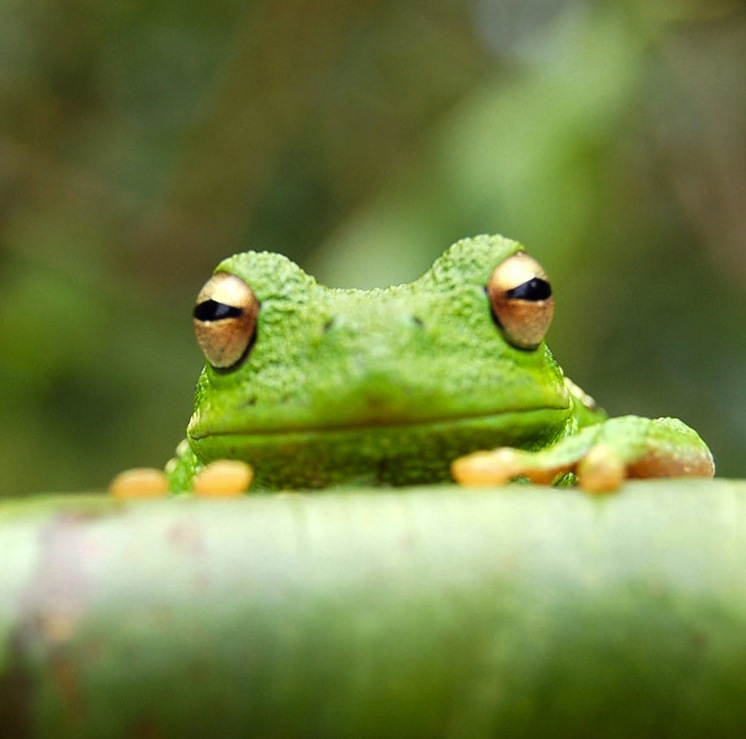
\includegraphics[width=0.2\textwidth]{frog.jpg}\\%\\[0.1in]
\vspace{3em}%
% Title
\Large \textbf {Cybersecurity deepfake placeholder}\\%\\[0.5in]
\vspace{1em}%
\normalsize by \\%
\vspace{1em}
\textup{\small {\bf Giorgio Mocci \\ Marco Motamed}\\}
 \vspace{1em}%
{\bf Laurea Magistrale in Ingegneria Informatica \\ Cybersecurity M}\\[0.5in]

\emph{\textbf{ABSTRACT} \\  A Project Report Submitted to the \\School of Computing and Informatics Technology
for the Study Leading to\\ a Project Report in Partial Fulfilment of the
requirements for the\\ Award of the Degree of Bachelor of Science in \\Computer Science
of Makerere University}

       % \small \emph{Submitted in partial fulfillment of\\
       %  the requirements for the award of the degree of}
        \vspace{1in}

       

% Submitted by
\normalsize {\bf Professore:} \\

[Michele Colajanni]\\
\vspace{1em}

% \begin{table}[h]
% \centering
% \begin{tabular}{lr}\hline \\
% Roll No & Names of Students \\ \\ \hline
% \\
% <Roll no here> & <Name here> \\
% <Roll no here> & <Name here> \\ 
% <Roll no here> & <Name here> \\ \\ \hline 
% \end{tabular}
% \end{table}

% \vspace{.1in}
% \date{}\\
% {\textbf{<Guide's name here>}}\\[0.2in]

\vfill

% Bottom of the page
% \includegraphics[width=0.18\textwidth]{./nitc-logo}\\[0.1in]
% \Large{Department of Computer Science and Engineering}\\
% \normalsize
% \textsc{National Institute of Technology Calicut}\\
% Calicut, Kerala, India -- 673 601 \\
% \vspace{0.2cm}
Dicembre , 2022

\end{center}

\end{titlepage}

\newpage

\section{Introduzione}
%obbiettivo report
Il seguente report ha come obiettivo l'analisi e lo studio dello stato dell'arte relativo alle tecniche, di cybersicurezza, per stabilire l'autenticità di un audio. \\\\
%descrizione tecnologie stato dell'arte 
Tramite l'utilizzo di reti neurali convoluzionali e dell'intelligenza artificiale si è ormai in grado di generare riproduzioni video e/o audio estremamente fedeli alla realtà. Fino a qualche anno fa tali strumenti risultavano essere accessibili solo ad un' "elite" di appassionati e ricercatori con accesso a macchine prestanti e con un'ampia conoscenza dell'argomento. Attualmente, in seguito al boom di queste tecnologie, queste tecniche sono applicabili da chiunque.
\\\\
%impatto sociale relativo
Nonostante queste tecnologie possano essere incredibilmente utili in molti ambiti, ad esempio medico, riabilitativo e sociale, è necessario interrogarsi sui problemi che un utilizzo improprio e scorretto possa causare nella società odierna.\\
Infatti, è possibile sintetizzare delle riproduzioni accurate senza il consenso dell'interessato andando a rubarne l'identità e utilizzandole per fini criminosi.
Queste riproduzioni risultano quasi impossibili da distinguere per l'utente comune e necessitano di ausili tecnologici esterni per essere individuate. \\
Per queste ragioni negli ultimi anni sono nati diversi modelli che, sfruttando il machine learning e l'intelligenza artificiale, permettono di riconoscere e una riproduzione generata artificialmente. 
\\\\
%Come è strutturato il report
Il documento è diviso in tre sezioni sintetizzati come di seguito: 
\begin{enumerate}
    \item Che cos'è un deepfake? Problemi nella società moderna
    \item Come individuare un deepfake (casi studio)
    \item Sperimentazione e lavoro svolto
\end{enumerate}


\pagenumbering{arabic} %reset numbering to normal for the main content


\newpage
\section{Usi e abusi del Deepfake}
%Descrizione deepfake
Il termine deepfake è utilizzato per indicare una riproduzione digitale (foto, video, audio), estremamente realistica, di una persona, animale, macchina o oggetto animato creata al fine di ingannare il fruitore rappresentando una realtà falsa costruita artificialmente.\\\\
%Origine del termine e settori
La parola deepfake è stata utilizzata per la prima volta nel 2017 da un utente di Reddit per riferirsi al software, da lui utilizzato, per creare filmati che partendo da video esistenti a sfondo sessuale andavano a modificare il volto dell'attrice con quello di una celebrità\cite{OrigineDeepfake}. 
\\
\begin{wrapfigure}{l}{0.35\textwidth}
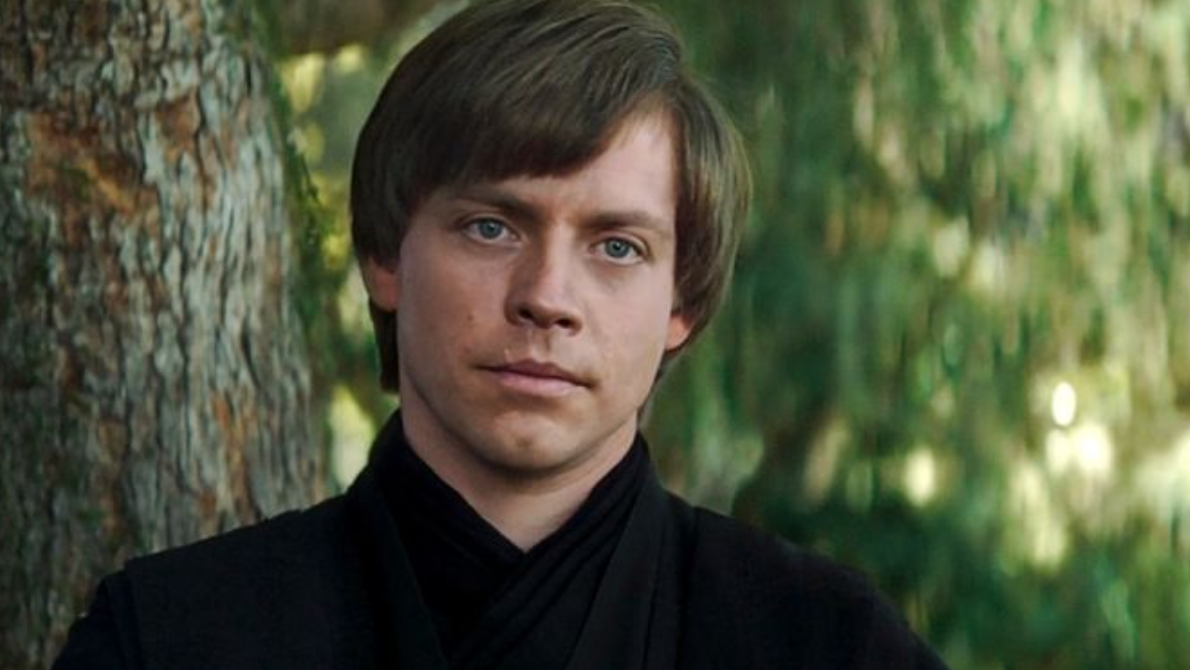
\includegraphics[width=1\linewidth]{Luke}
\caption{Frame del film "The Book of Boba Fett" rappresentante una riproduzione deepfake dell'attore Mark Hamill nelle vesti del giovane Luke Skywalker}
\label{fig:wrapfig}
\end{wrapfigure}
Da allora il termine deepfake si è evoluto e ha anche assunto una parziale accezione positiva. Infatti, grazie a questa tecnologia è possibile creare materiale a supporto di numerosi nobili settori, come ad esempio quello medico, cinematografico ed educativo.\cite{LukeDeepfake}\\
Un altro esempio rilevante può essere l'assistenza alle persone che, in seguito alla perdita di un proprio caro, possono giovare di queste riproduzioni per aiutarle a superare il loro trauma\cite{SuperareTrauma}.
\\\\
%Problemi sociale correlati al deepfake
Purtroppo però, la stragrande maggioranza dei deepfake sono utilizzati in maniera dannosa, con lo scopo di screditare un personaggio pubblico, di mortificare e umiliare un individuo (solitamente tramite video pornografici che colpiscono maggiormente target femminili) o deviare l'opinione pubblica verso un determinato obiettivo in maniera similare a quanto avviene con le fakenews.
\\
Un possibile esempio di come questi utilizzi possano diventare di importanza nazionale è quanto accaduto nel 2019 alla allora "house speaker" Nancy Pelosi, dove un video di questo tipo la ritraeva visibilmente alterata come se fosse in preda ai fumi dell'alcol\cite{FakeVideoNancyPelosi}.
\\\\%conclusione capitolo
Appare evidente come un utilizzo scorretto di queste tecnologie possa provocare ingenti danni economici e sociali alla collettività. Risulta quindi imperativa una maggiore attenzione da parte del governo e dell'opinione pubblica sull'argomento, al fine di sensibilizzare la popolazione e le aziende del settore in modo da per poter combattere efficacemente questa crescente piaga.



\newpage

\section{Come possiamo individuare un deepfake?}
%Tecniche per riconoscerli da un punto di vista umano/sociale
In questo capitolo verranno trattate le tecniche che possono essere usate per distinguere un video genuino da uno fasullo.\\ La prima categoria riguarda le metodologie basate sul riconoscimento di difetti e pattern comuni ai video deepfake.\\\\
Ad esempio una caratteristica comune ai suddetti video è la gestione innaturale degli occhi. Infatti, i soggetti sbattono le palpebre troppo spesso o troppo di rado o in casi estremi non le sbattono affatto.\\
Questo e altri simili problemi possono essere utili ad individuare riproduzioni sbrigative o poco curate. Purtroppo quelle di ultima generazione non presentano più queste problematiche ed è quindi necessario affidarsi a strumenti più sofisticati per raggiungere lo scopo.\\\\
%Tecniche per riconoscerli da un punto di vista scientifico
Tramite l'utilizzo di tecniche basate su machine learning e intelligenza artificiale è possibile realizzare modelli in grado di individuare, con un certo grado di attendibilità, la maggior parte delle riproduzioni deepfake. Ultimamente, però, sono emerse nuove metodologie in grado di ingannare questi strumenti.\\
Un celebre esempio è GANs, una rete neurale in grado di riconoscere automaticamente le possibili falle e migliorare la generazione del deepfake attraverso molteplici round, rendendo estremamente difficili l'individuazione da parte di software appositi.\\\\
%Caso di studio(Minerva, Intel, Who are you...)
Ovviamente anche gli esperti di cybersecurity hanno migliorato i propri sistemi, attraverso nuove tecniche che vanno a concentrarsi su parametri più specifici e precisi che attualmente risultano estremamente complessi da emulare.\\
\begin{wrapfigure}{l}{0.55 \textwidth}
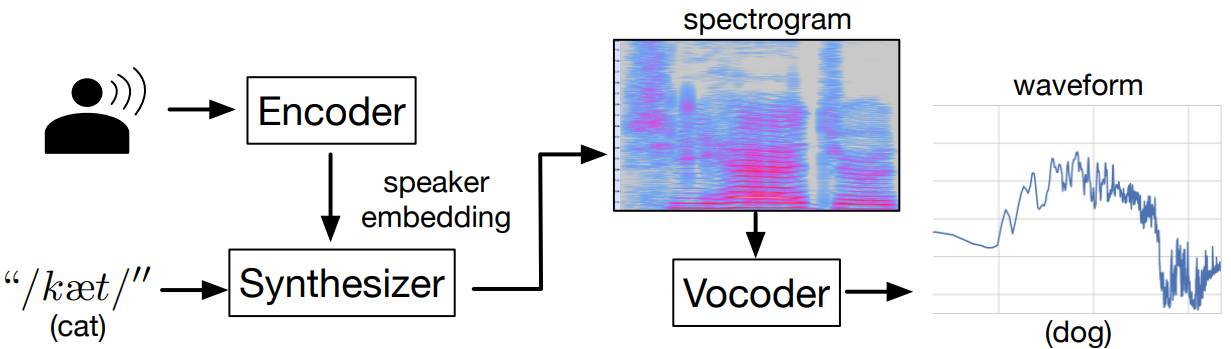
\includegraphics[width=1\linewidth]{waveform.png}
\caption{L'encoder incapsula l'audio del soggetto, il sintetizzatore crea uno spettrogramma perla frase obbiettivo usando l'incapsulamento precedente e il vocoder converte lo spettrogramma nella forma d'onda sintetica.}
\label{fig2:wrapfig}
\end{wrapfigure}
Un esempio virtuoso è il software sviluppato dai ricercatori dell'università della Florida, Gainesville in grado di riconoscere i deepfake audio utilizzando una tecnica basata sull'analisi dell' impronta generata dalle corde vocali \cite{280020}. \\\\\\
\newpage
Un'altra interessante tecnologia è quella sviluppata da Intel, in grado di individuare i deepfake video tramite deep-learning e lo studio dei flussi sanguigni attraverso i vasi della testa.\\
Intel dichiara un'accuratezza di individuazione del 96\% e promette di generare un risultato in pochi millisecondi, rendendo il servizio utilizzabile anche per l'analisi real-time di un video.\cite{DBLP:journals/corr/abs-1901-02212} \\\\
\begin{figure}[h]
    \centering
    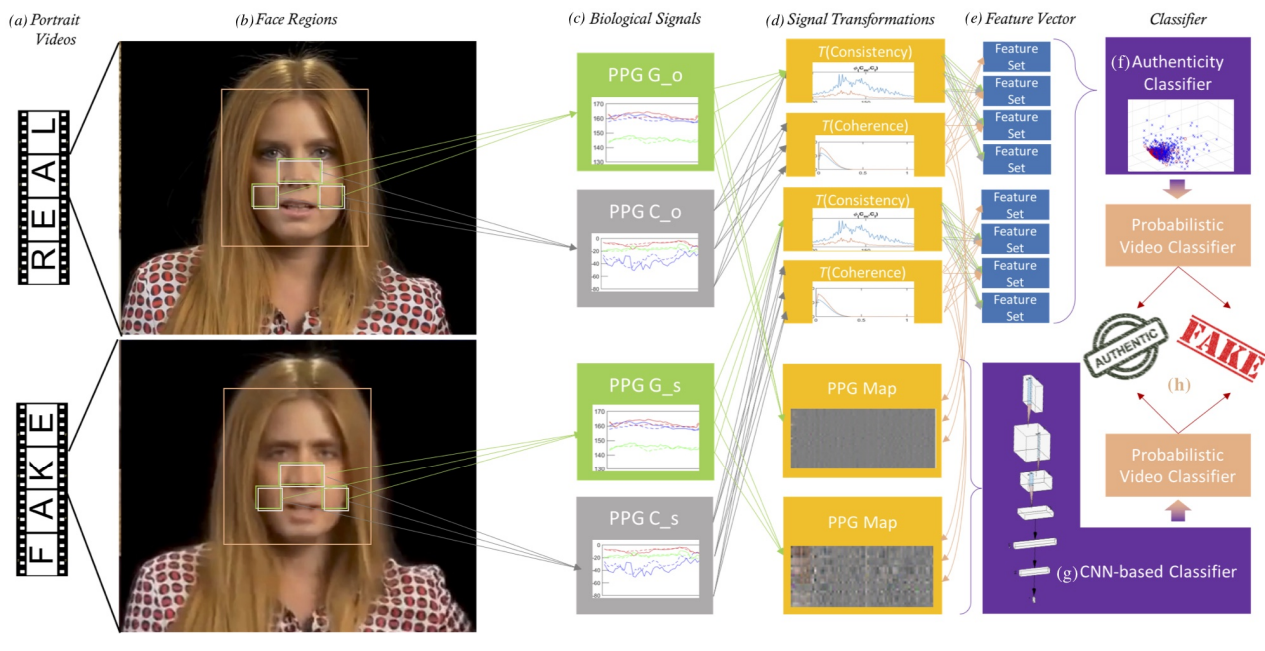
\includegraphics[width=1\textwidth]{bloodDetector.png}
    \caption{Partendo da una coppia reale e fake di frame(a) sono stati estratti segnali biologici (c) da diverse regioni facciali (b). Sono state applicate transformazioni (d) per calcolare coerenza spaizale e consistenza temporale, catturando segnali caratteristici(e) in un set di label e PPG maps e utilizzandoli per addestrare modelli di apprendimento SVM (f) e CNN (g). Infine vengono calcolate le probabilità (h) per stabilire l'autenticità dei frame iniziali (a). }
    \label{fig:mesh1}
\end{figure} \\
Purtroppo questi software non sono stati ancora resi disponibili e risultano impossibili da testare. Per questo motivo nel prossimo capitolo verrà trattato il nostro personale approccio a questa problematica.
\newpage
\section{Il nostro modello per il deepfake's audio detection}
In questo capitolo verrà presentato il nostro modello di individuazione degli audio deepfake. \\
Per le motivazioni trattate nel precedente capitolo abbiamo deciso di sviluppare uno strumento che ci permettesse di effettuare test personalizzati approfondendo la problematica da un punto di vista più pratico.\\
A tal fine abbiamo addestrato una rete neurale convoluzionale. Questa tecnologia, emulando il funzionamento del nostro cervello e partendo da una base di dati, riesce attraverso diversi livelli a predire un risultato. \\\\
Per quanto riguarda la base di dati ci siamo affidati ai dataset di ASVspoof per gli audio fake \cite{FakeAudioDataset} e a Common Voice per gli audio genuini \cite{RealAudioDataset}.
Per poter utilizzare questi file è stato necessario estrarre dagli audio i coefficienti Mel-frequency cestral (rappresentazione spettro di potenza a breve termine di un suono)\\
\begin{code}
\captionof*{code}{Procedura di estrazione MFCC}
\label{code:python-code}
\begin{pythoncode}{c}
def features_extractor(file_name):
    audio, sample_rate = librosa.load(file_name, res_type= 'kaiser_fast') 
    mfccs_features = librosa.feature.mfcc(y=audio, sr=sample_rate, n_mfcc=40)
    mfccs_scaled_features = np.mean(mfccs_features.T,axis=0) 
    return mfccs_scaled_features  
\end{pythoncode}
\end{code}
% ----------------------------------------------
\begin{figure}[h]
    \centering
    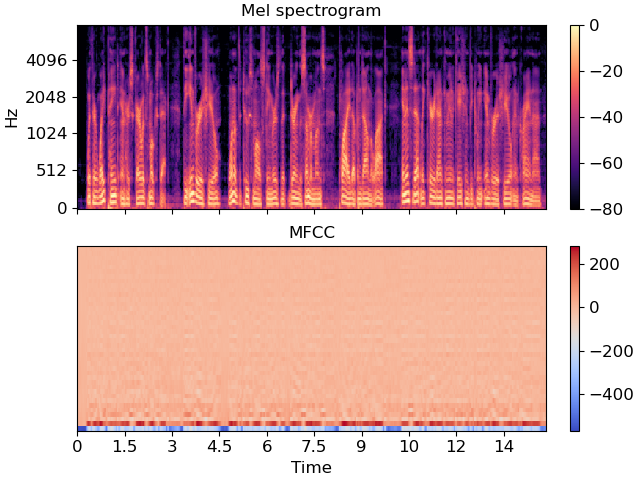
\includegraphics[width=0.7\textwidth]{librosa-feature-mfcc-1_00.png}
    \caption{Esempio di spettrogramma MEl e relativo MFCC }
\end{figure} 
% addestramento rete, parametri importanti, foto risultati e prestazioni ottenute
Per il training del modello ci siamo affidati al framework di tensorflow.keras utilizzando una gpu Geforce Rtx 2060. Dopo una serie di test abbiamo constato che l'addestramento sequenziale fosse il più adatto alle nostre esigenze. Infatti, tale metodologia ci ha permesso di sfruttare al meglio le informazioni in nostro possesso ottenendo una maggiore accuratezza e precisione.\\
Di seguito vengono riportati i parametri che riteniamo essere più rilevanti ed i risultati ottenuti a seguito dell'addestramento della rete. 
% ----------------------------------------------
\begin{code}
\captionof*{code}{Parametri utilizzati nell'addestramento}
\label{code:python-code}
\begin{pythoncode}{c}
model.compile(loss='categorical_crossentropy',metrics=['accuracy'],optimizer='adam')
lr_reduction = ReduceLROnPlateau(monitor = 'val_loss',patience = 3,verbose = 1,factor = 0.2
                                ,min_lr = 0.001)
callbacks = [lr_reduction]
num_epochs = 50
num_batch_size = 32
history = model.fit(X_train,
          y_train,
          batch_size=num_batch_size,
          epochs=num_epochs,
          validation_data=(X_val, y_val),
          callbacks=callbacks,
          verbose=1)
\end{pythoncode}
\end{code}
%Modalità di funzionamento(come fa a capire che un audio è fake o no
%Foto risultati ottenuti e descrizione caratteristiche e considerazioni finali.
% ----------------------------------------------
\begin{minipage}{0.4\textwidth}
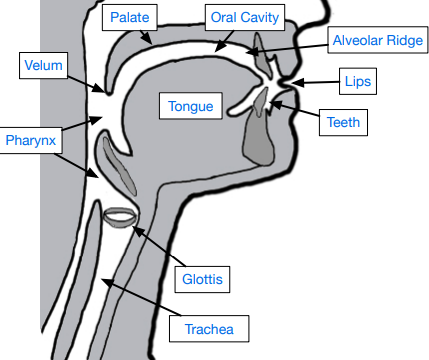
\includegraphics[width=\linewidth]{VocalBiologicalTraits.png}
\end{minipage}
\begin{minipage}{0.6\textwidth}
I risultati restituiti si basano sulle divergenze esistenti tra gli audio reali, che sono limitati dalla struttura organica delle corde vocali, e gli audio deepfake \textit{GAN-generated} che non hanno queste limitazioni. Il tratto vocale è composto da vari componenti che agiscono insieme per produrre un suono. I distinti suoni sono articolati in base al percorso dell'aria, che è determinato da come sono posizioni i componenti \cite{280020}.\\
\end{minipage}
\\
In conclusione ci riteniamo soddisfatti dei risultati ottenuti. Abbiamo scelto di rendere diffidente il nostro riconoscitore, in caso non sia certo del risultato predetto, in modo da evitare il più possibile i falsi positivi.\\ 
Il nostro modello riesce a raggiungere una precisione superiore al 95\% con gli audio appartenenti alla stessa tipologia dei dataset utilizzati durante l'addestramento; mentre ha più difficoltà a riconoscere i deepfake generati con altre tecnologie.\\
Questa problematica verrà approfondita nel prossimo ed ultimo capitolo.
\newpage
\section{Conclusione}






\newpage
\bibliographystyle{unsrt}
\bibliography{bibliography}

\end{document}
